\section{Diagrammi dei package}
\begin{figure}[hb]
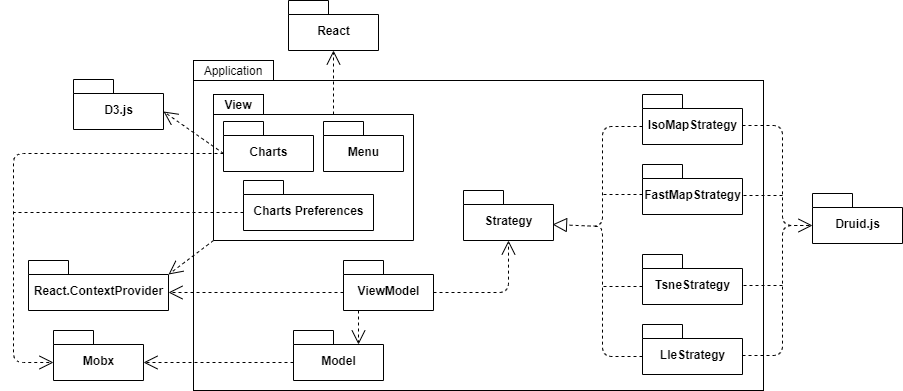
\includegraphics[width=15.8cm]{Images/Allegato Tecnico-Package}
\centering
\caption{Diagramma dei package client side}
\end{figure}

Il diagramma sopra riportato descrive a livello di package le parti che compongono il lato client dell'applicazione. In particolare si può notare come \textit{View} e \textit{Model} non siano direttamente collegati, ma il passaggio delle informazioni avviene attraverso il \textit{ViewModel} e il componente \glo{\textit{Context Provider}} fornito da React. \\ %componente fornito da React per consumare il contesto creato

%\begin{figure}[hb]
%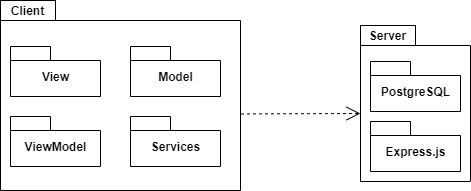
\includegraphics[width=15.8cm]{Images/Allegato Tecnico-Package 2}
%\centering
%\caption{Connessione tra client side e server side}
%\end{figure}
